\documentclass[border=.1cm]{standalone}

\usepackage{tikz}
\usepackage{times}
\usepackage{pgfplots}
\usepgflibrary{arrows}

\usepackage{siunitx}
\sisetup{
    detect-all = true,
    input-decimal-markers = {.},
    input-ignore = {,},
    inter-unit-product = \ensuremath{{}\cdot{}},
    multi-part-units = repeat,
    number-unit-product = \text{~},
    per-mode = fraction,
    separate-uncertainty = true,
}

\begin{document}

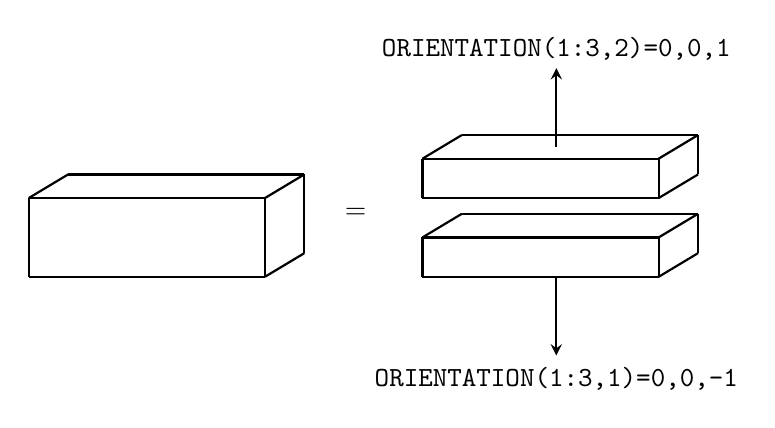
\begin{tikzpicture}

\draw [thick]  (0,0) -- (0,1);
\draw [thick]  (0,0) -- (3,0);
\draw [thick]  (3,0) -- (3,1);
\draw [thick]  (0,1) -- (3,1);
\draw [thick]  (0,1) -- (.5,1.3);
\draw [thick]  (.5,1.3) -- (3.5,1.3);
\draw [thick]  (3,1) -- (3.5,1.3);
\draw [thick]  (3.5,1.3) -- (3.5,.3);
\draw [thick]  (3,0) -- (3.5,.3);

\draw [thick]  (5,0) -- (5,.5);
\draw [thick]  (5,0) -- (8,0);
\draw [thick]  (8,0) -- (8,.5);
\draw [thick]  (5,.5) -- (8,.5);
\draw [thick]  (5,.5) -- (5.5,.8);
\draw [thick]  (5.5,.8) -- (8.5,.8);
\draw [thick]  (8,.5) -- (8.5,.8);
\draw [thick]  (8.5,.8) -- (8.5,.3);
\draw [thick]  (8,0) -- (8.5,.3);
\draw [-stealth, thick]  (6.7,0) -- (6.7,-1);
\node at (6.7,-1.3) {\tt ORIENTATION(1:3,1)=0,0,-1};

\draw [thick]  (5,1) -- (5,1.5);
\draw [thick]  (5,1) -- (8,1);
\draw [thick]  (8,1) -- (8,1.5);
\draw [thick]  (5,1.5) -- (8,1.5);
\draw [thick]  (5,1.5) -- (5.5,1.8);
\draw [thick]  (5.5,1.8) -- (8.5,1.8);
\draw [thick]  (8,1.5) -- (8.5,1.8);
\draw [thick]  (8.5,1.8) -- (8.5,1.3);
\draw [thick]  (8,1) -- (8.5,1.3);
\draw [-stealth, thick]  (6.7,1.65) -- (6.7,2.65);
\node at (6.7,2.9) {\tt ORIENTATION(1:3,2)=0,0,1};

\node at (4.15,.8) {=};

\end{tikzpicture}

\end{document}
